
{\setbeamertemplate{footline}{}
\begin{frame}[noframenumbering]
		\titlepage
\end{frame}
}

\begin{frame}{Параллельная обработка данных}
	В мире существует множество задач, требующих параллельной обработки данных:
	\begin{itemize}
		\item Параллельные вычисления. Например, библиотека Colt Parallel, используемая CERN для математических расчетов.
		\item Системы сбора и обработки данных.
	\end{itemize}
\end{frame}

\begin{frame}{Система обработки и сбора данных}
	\begin{figure}
		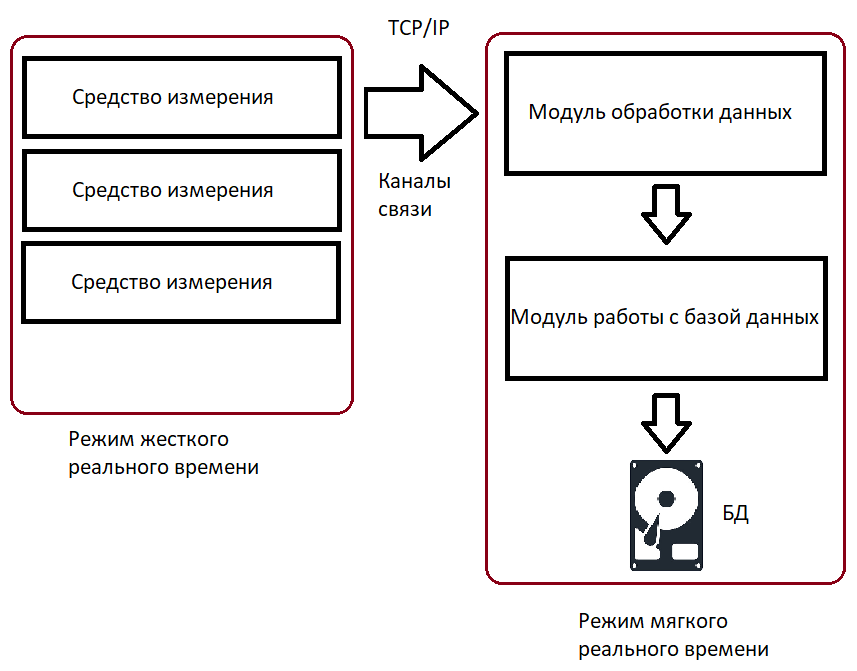
\includegraphics[width=0.9\linewidth]{images/system.png}
	\end{figure}
	\begin{itemize}
		\item Для ускорения работы со множеством каналов связи необходим параллелизм.
	\end{itemize}
\end{frame}

\begin{frame}{Язык Java}
	\begin{enumerate}
		\item Допустимо применение языка Java в системах мягкого реального времени.
		\item Java упрощает написание кода благодаря автоматическому управлению памятью 
		и контролю ошибок при исполнении. 
\end{enumerate}
\end{frame}

\begin{frame}{Параллелизм}
	\begin{itemize}
	\item Традиционно, параллелизм реализуется внутри операционной системы с помощью механизма потоков.
	\item Однако, модель потоков имеет ряд минусов. 
	\item Потоки -- это достаточно "тяжеловесный" механизм: их создание и переключение несет в себе крупные накладные расходы. 
	\item Избежать накладных расходов на использование потоков можно, применяя вместо них сопрограммы. 
	\end{itemize}
\end{frame}

\begin{frame}{Сопрограммы}
	\begin{itemize}
		\item \textbf{Сопрограмма} (англ. coroutine) - программный модуль, который работает 
		\textit{конкурентно} с другими такими модулями. При использовании сопрограммы ведут себя как обычные потоки.
		
		\item Сопрограммы уже реализованы в языках программирования С++20, C\#, Go.
		\item Модуль сопрограмм в Java находится в стадии работающего прототипа (OpenJDK/Loom)
	\end{itemize}
\end{frame}

\begin{frame}{Цели и задачи}
	Цель: изучение применимости сопрограмм вместо потоков в параллельных системах.
	\par
	Поставленные задачи:
	\begin{itemize}
		\item Провести анализ реализаций сопрограмм в других языках.
		\item Реализовать прототип модуля сопрограмм.
		\item Сравнить производительность сопрограмм и потоков.
		\item Выявить ключевые плюсы использования сопрограмм.
	\end{itemize}
	Работа проводится на базе Huawei JDK.
\end{frame} 

\begin{frame}{Анализ реализаций}
	Был создан набор тестов производительности сопрограмм для языков Go, Java (с “Loom Project”).
	
	Тесты создавались для измерения 2 параметров.
	\begin{enumerate}
		\item Скорость переключения контекста.
		\item Потребление памяти.
	\end{enumerate}
	\begin{itemize}
		\item Разработанные тесты позволят оценить применимость сопрограмм в системах сбора данных.
		\item Репозиторий с тестами: https://github.com/minium2/coroutines-benchmark.
	\end{itemize}
\end{frame}

\begin{frame}{Реализация прототипа сопрограмм}
	Для работы минимального прототипа требуется:
	\begin{enumerate}
		\item Переключение контекста сопрограмм.
		\item Сборка мусора.
	\end{enumerate}
	Переключение сопрограмм может быть реализовано различными способами:
	\begin{itemize}
		\item OpenJDK/Loom: копирование стека сопрограммы при переключении.
		\item Go: изменение указателя стека.
	\end{itemize}
	В HuaweiJDK выбран подход языка Go, поскольку он более эффективен.
\end{frame}

\begin{frame}{Измерение скорости переключения сопрограмм в управляемых средах}
	Ubuntu, kernel 4.15, Intel Core i7-8700, 4.6 ГГц, 32 Гб ОЗУ
	\par Каждое значение усреднено по 100 измерениям. 
	
	\begin{table}[H]
		%\caption{Число переключений корутин}\label{inc-matrix}
		\textit{\begin{tabular}{|c|c|c|c|c|c|}
				\hline \multirow{2}{*}{Шт.} & \multicolumn{3}{|c|}{Число переключений, тыс./сек.}                  \\
				\cline{2-4}               & HuaweiJDK                  & OpenJDK/"Loom"     & Go                   \\
				\hline 100                & \numprint{12980} $\pm$ 540 & \numprint{1900} $\pm$ 20\phantom{0}    & \numprint{18187} $\pm$ 219 \\
				\hline \numprint{1000}    & \numprint{11420} $\pm$ 694 & \numprint{1775} $\pm$ 20\phantom{0}    & \numprint{17934} $\pm$ 332 \\
				\hline \numprint{5000}    & \phantom{0}\numprint{5875} $\pm$ 183   & \numprint{1703} $\pm$ 30\phantom{0}    & \numprint{12892} $\pm$ 339 \\  
				\hline \numprint{10000}   & \phantom{0}\numprint{4459} $\pm$ 162 & \numprint{1924} $\pm$ 235  & \numprint{8307} $\pm$ 80   \\  
				\hline \numprint{20000}   & \numprint{3604} $\pm$ 93 & \numprint{1863} $\pm$ 217   			  & \numprint{7045} $\pm$ 72   \\ 
				\hline \numprint{30000}   & \numprint{3031} $\pm$ 94 & \numprint{1772} $\pm$ 182   			  & \numprint{6391} $\pm$ 94   \\ 
				\hline \numprint{40000}   & \numprint{2653} $\pm$ 87 & \numprint{1606} $\pm$ 194              & \numprint{5790} $\pm$ 67   \\ 
				\hline \numprint{50000}   & \numprint{2315} $\pm$ 60 & \numprint{1503} $\pm$ 157              & \phantom{0}\numprint{5292} $\pm$ 122  \\  
				\hline 
		\end{tabular}}
	\end{table}	
\end{frame}

\begin{frame}{Измерение скорости переключения потоков и сопрограмм}
	Ubuntu, kernel 4.15, Intel Core i7-8700, 4.6 ГГц, 32 Гб ОЗУ, HuaweiJDK
	\par Каждое значение усреднено по 100 измерениям. 
	\par Для измерения используется только одно ядро ЦП.
	\begin{table}[H]
		%\caption{Число переключений корутин}\label{inc-matrix}
		\textit{\begin{tabular}{|c|c|c|c|c|c|}
				\hline \multirow{2}{*}{Шт.} & \multicolumn{2}{|c|}{Число переключений, тыс./сек.} \\
				\cline{2-3}              & Сопрограммы                           & Потоки                    \\
				\hline 100               & \numprint{12980} $\pm$ 540            & \numprint{2306} $\pm$ 50  \\
				\hline \numprint{1000}   & \numprint{11420} $\pm$ 694            & \numprint{2300} $\pm$ 27  \\
				\hline \numprint{5000}   & \phantom{0}\numprint{5875} $\pm$ 183  & \numprint{1554} $\pm$ 37   \\
				\hline \numprint{10000}  & \phantom{0}\numprint{4459} $\pm$ 162  & \numprint{1016} $\pm$ 29   \\ 
				\hline \numprint{20000}  & \numprint{3604} $\pm$ 93              & \phantom{0}753   $\pm$ 28              \\ 
				\hline \numprint{30000}  & \numprint{3031} $\pm$ 94              & \phantom{0}556   $\pm$ 16              \\ 
				\hline \numprint{40000}  & \numprint{2653} $\pm$ 87              & \phantom{0}436   $\pm$ 12              \\ 
				\hline \numprint{50000}  & \numprint{2315} $\pm$ 60              & 		      361   $\pm$ 8               \\ 
				\hline 
			\end{tabular}
		}
	\end{table}
\end{frame}

\begin{frame}{Измерение потребление памяти сопрограмм в управляемых средах}
	Ubuntu, kernel 4.15, Intel Core i7-8700, 4.6 ГГц, 32 Гб ОЗУ
	\begin{table}[H]
		\textit{\begin{tabular}{|c|c|c|c|c|c|}
			\hline \multirow{2}{*}{Шт.} & \multicolumn{4}{|c|}{Резидентная память}  \\
			\cline{2-5}    & HuaweiJDK   & OpenJDK/"Loom"    & Go       & Потоки \\
			\hline 100     & 18 Mб       & 130 Mб    		 & 3,040 Mб & 34 Mб \\
			\hline 1000    & 22 Mб       & 161 Mб     		 & 3,105 Mб & 35 Mб \\
			\hline 5000    & 32 Mб       & 187 Mб    		 & 3,156 Mб & 37 Mб \\
			\hline 10000   & 37 Mб       & 193 Mб     		 & 3,308 Mб & 40 Mб \\
			\hline 20000   & 45 Mб       & 196 Mб     		 & 3,320 Mб & 49 Mб \\
			\hline 30000   & 49 Mб       & 197 Mб     		 & 3,350 Mб & 56 Mб \\
			\hline 40000   & 51 Mб       & 200 Mб    		 & 3,390 Mб & 63 Mб \\
			\hline 50000   & 57 Mб       & 202 Mб    		 & 3,407 Mб & 72 Mб \\ 
			\hline 
		\end{tabular}}
	\end{table}
\end{frame}

\begin{frame}{Вычислительные задачи}
	Для измерений была применена библиотека Colt Parallel и
	ее вариант на сопрограммаах OpenJDK/Loom.
	\begin{table}[H]
		Время перемножения матриц 6000x7000
		\begin{tabular}{|c|c|} 
			\hline Потоки              & Сопрограммы         \\
			\hline 45.6 $\pm$ 1.8 сек. & 24.0 $\pm$ 5.6 сек. \\ 
			\hline
		\end{tabular}
	\end{table}
	\begin{table}[H]
		Время вычисления дискретного преобразования Фурье.
		\begin{tabular}{|c|c|} 
			\hline Потоки                 & Сопрограммы         \\
			\hline 77.2 $\pm$ 0.3 мсек.   & 77.4 $\pm$ 0.4 мсек.\\ 
			\hline
		\end{tabular}
	\end{table}
	Измерения проводились на CentOS, linux 4.18.0 Intel$^{\textregistered}$  Xeon$^{\textregistered}$ Gold 6130, 2.10 ГГц.
\end{frame}

\begin{frame}{Ключевые отличия от потоков ОС}
	\begin{itemize}
		\item Переключение контекста сопрограммы требует меньше накладных расходов, чем потока. Измерено: скорость переключения сопрограмм в 5--7 раз больше, чем у потоков.
		\item Меньшее потребление физической памяти более, чем на 20\%.
	\end{itemize}
\end{frame}

\begin{frame}{План дальнейших работ} 
	\begin{itemize}
		\item Реализовать переключение сопрограммы при вызове ввода--вывода.
		\item Оценить реальный рост производительности от применения сопрограмм в системах обработки данных.
	\end{itemize}
\end{frame}

\begin{frame}{Результаты}
	\begin{itemize}
		\item Создан набор тестов для сравнения производительности потоков и сопрограмм.
		\item Реализован базовый прототип сопрограмм на базе HuaweiJDK.
		\item Проведен анализ результатов тестов производительности.
		\item Выявлены ключевые отличия сопрограмм от потоков. Можно ожидать прирост
		производительности при использовании сопрограмм в системах сбора данных.
	\end{itemize}
\end{frame}

